\section{Foundations of Data Flow Analysis}



We saw a lot of examples of data flow analysis, eg. reaching definitions etc. Although 
there were differences between differeent types of data flow analysis, they did share number of 
things in common. Our goal is to develop a general purpose data flow analysis framework.


There are some questions that we want to answer about a framework that performs data 
flow analysis.

\begin{itemize}
\item Correctness: Do we get a correct answer? 
\item Precison: How good is the answer? \footnote{We want a safe solution but as precise as possible. }
\item Covergence: Will the analysis terminate? 
\item Spped: How fast is the convergence?
\end{itemize}



\subsection{A Unified Framework}

Data flow problems are defined by 
\begin{itemize}

\item Domain of values \( V \)(eg, variable names for liverness, the instruction numbers for reaching definitions)
\item Meet operator \( V \wedge V \rightarrow V \) to deal with the join nodes.
\item Initial value. Once we have defined the meet operator, it will tell us how to initialize 
all of the non-entry or exits nodes and the boundary conditions for entry and exit nodes. 
\item A set of transfer functions \( V  \rightarrow V \) to define how information flows across basic blocks. 
\end{itemize}   



Why we bother to define such a framework?
\begin{itemize}
\item First, if meet operator, transfer function and the domains of values are specified in proper way, we will know about 
correctness, precision and so on. 

\item From prectical engineering perspective, it allows us to reuse code.
\end{itemize}   


\subsection{Partial Order}

A relation \(R\) on a set \(S\) is called a \textbf{partial order} if it is

\begin{itemize}
    \item \textbf{Transitivity} if \(x \preceq y\) and  \(y \preceq z\) then  \(x \preceq z\)
    \item \textbf{Antisymmetriy} if \(x \preceq y\) and  \(y \preceq x\) then  \(x = z\)
    \item \textbf{Reflexivity}  \(x = x\)
\end{itemize}    

\subsection{Lattice}

A lattice is a partially ordered set in which every pair of elements has both a least upper bound (lub)
 and a greatest lower bound(glb). 

\begin{figure}[h]
    \centering
    \begin{subfigure}[b]{0.3\textwidth}
        \centering
        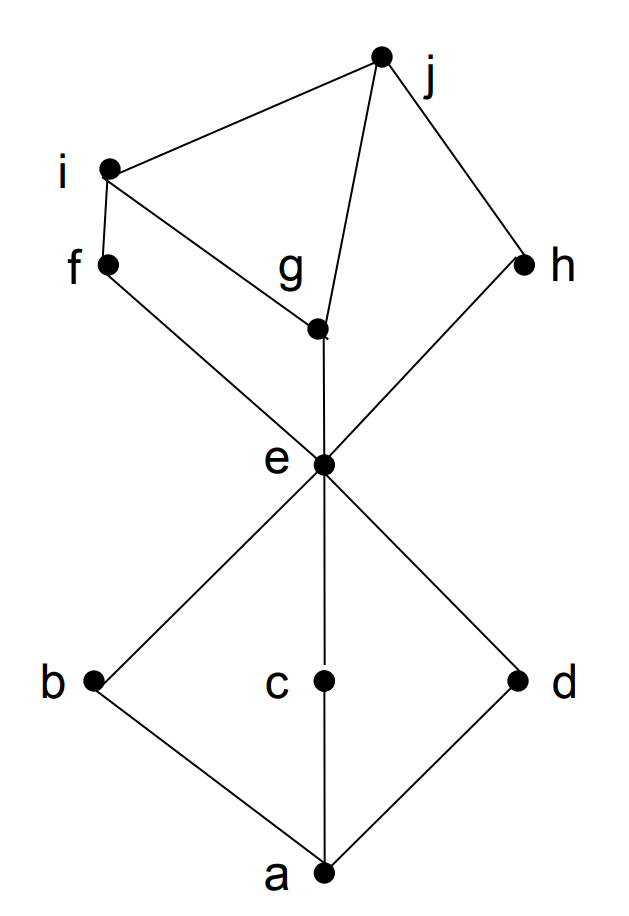
\includegraphics[width=\textwidth]{p17.png}
        \caption{This is a lattice example.}
        \label{fig:p17}
    \end{subfigure}
    \hfill
    \begin{subfigure}[b]{0.3\textwidth}
        \centering
        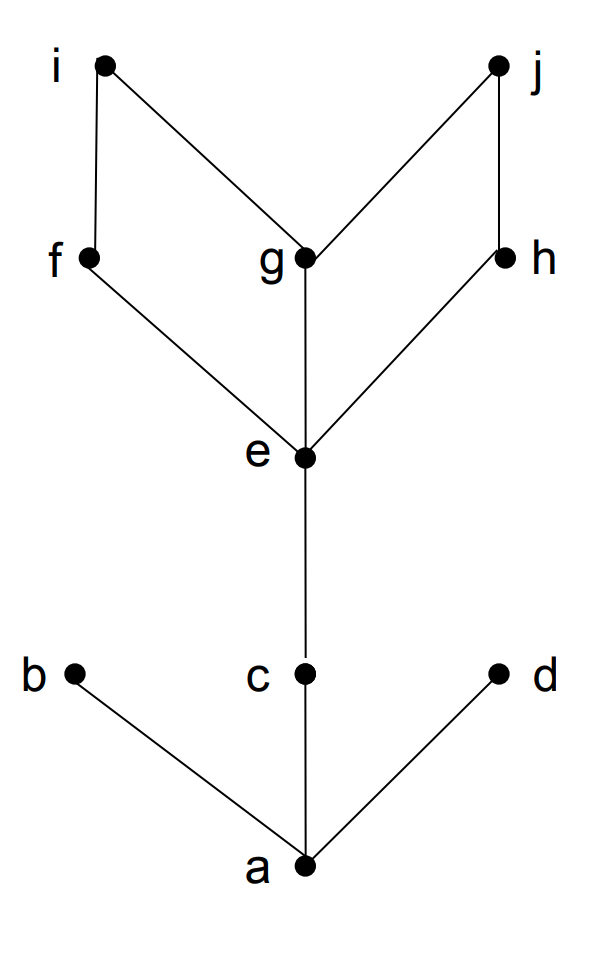
\includegraphics[width=\textwidth]{p16.png}
        \caption{This is not a lattice example becuasethe pair {b,c} deos not have a lub.}
        \label{fig:three sin x}
    \end{subfigure}
       \caption{Two examples}
       \label{fig:p16}
\end{figure}





\subsection{Complete Lattice}

A lattice A is called a complete lattice if every subset S of A admits a
glb and a lub in A.



\subsection{Semi-Lattice}

A semilattice (or upper semilattice) is a partially ordered set that has a least upper bound for any 
nonempty finite subset.





\subsection{ Meet Operator }

Meet operator must hold the following properties:

\begin{itemize}
\item \textbf{commutative}: \(x \wedge y = y = \wedge x\). No ordering in the incoming edges.

\item \textbf{idempotent}: \(x \wedge x =  x\)

\item \textbf{associative }: \(x \wedge( y\wedge z) =  (x \wedge y) \wedge z\)

\item there is a Top element T such that \(x \wedge T = x\). Partly due to the way 
we initialize everything we need.
\end{itemize}

\begin{figure}[h]
    \centering
    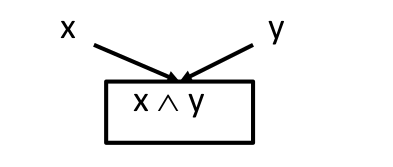
\includegraphics[width=0.3\textwidth]{p15.png}
    \caption{Meet Operator}
    \label{fig:p15}
\end{figure}



Meet Operator defines a partial ordering on values. This is important in ensuring the analysis converges. So 
what does it mean ? \(x \preceq y\) if and only if \(x \wedge y = x\). The \(\preceq \) not means less or equal to or subset, but it really means lattice inclusion.
So if \(x \preceq y\), this means x is more conservative or constrained. In another word, x is lattice included in y.
Partial  ordering will also lead to some other properties
    \begin{itemize}
        \item \textbf{Transitivity} if \(x \preceq y\) and  \(y \preceq z\) then  \(x \preceq z\)
        \item \textbf{Antisymmetriy} if \(x \preceq y\) and  \(y \preceq x\) then  \(x = z\)
        \item \textbf{Reflexivity}  \(x = x\)
\end{itemize}


\begin{figure}[h]
    \centering
    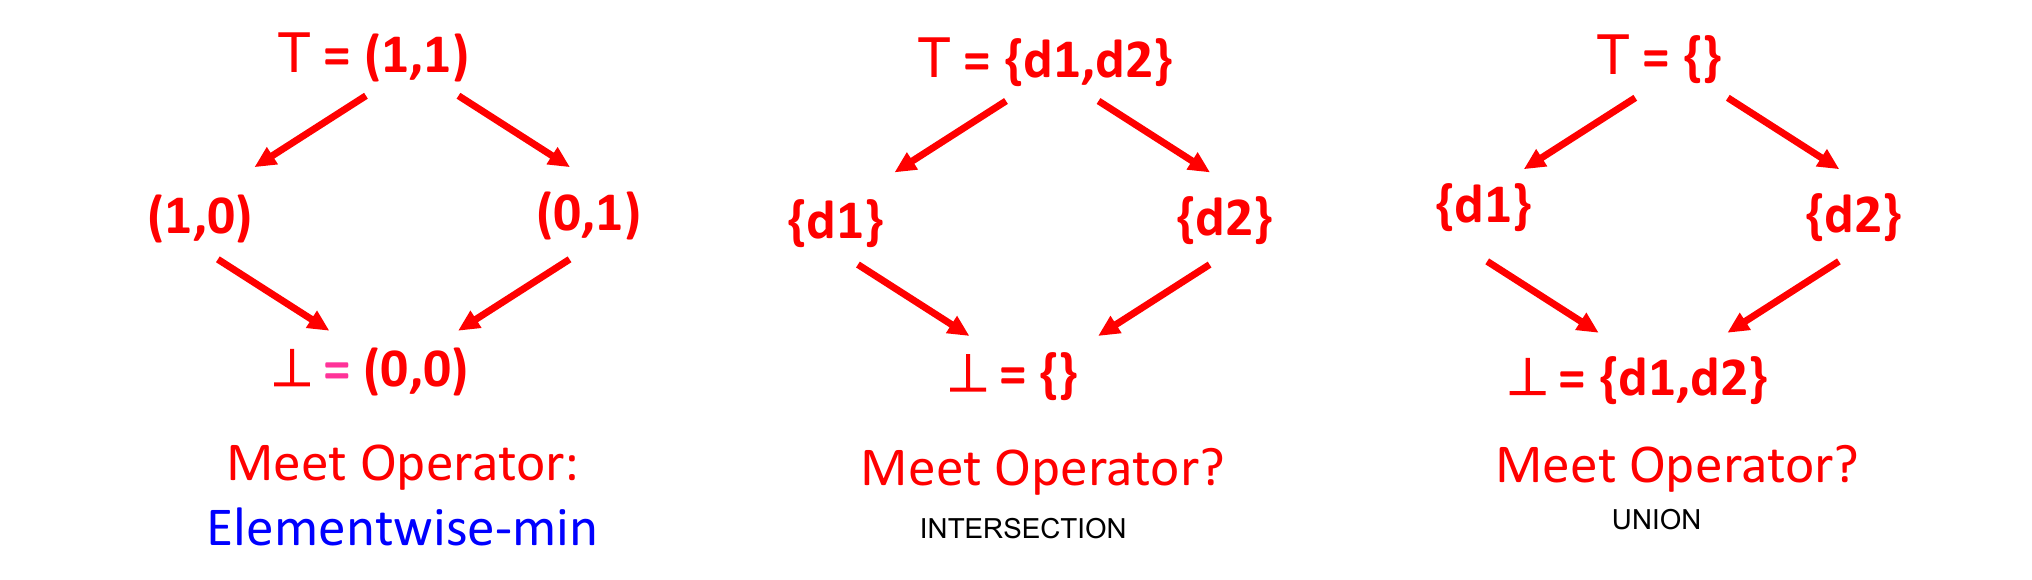
\includegraphics[width=\textwidth]{p18.png}
    \caption{Different meet operator defines different lattice}
    \label{fig:p15}
\end{figure}


% \subsection{Partial Order}


For our data flow analysis, values and meet operator define a semi-lattice, which means \(\top\) exits, but not necessarily \(	\bot\).





\subsection{Descending Chain}

The height of a lattice is the largest number of \(\succ \) relations that will fit in a descending chain. eg. \(x_0 \succ x_1 \succ x_2 \succ \dots\)

So, for reaching definitions, the height is the number of definitions.

Finite descending chain will ensure the convergence. If we don't finite descending chain, there is a possibility that
the analysis will never terminate. But a infinite lattice still can have a finite descending chain. I want to note that 
infinite lattice doesn't always mean a non-convergence.

So consider the constant propogation, the infinite lattice has finite descending chain, so this can converge.

\begin{figure}[h]
    \centering
    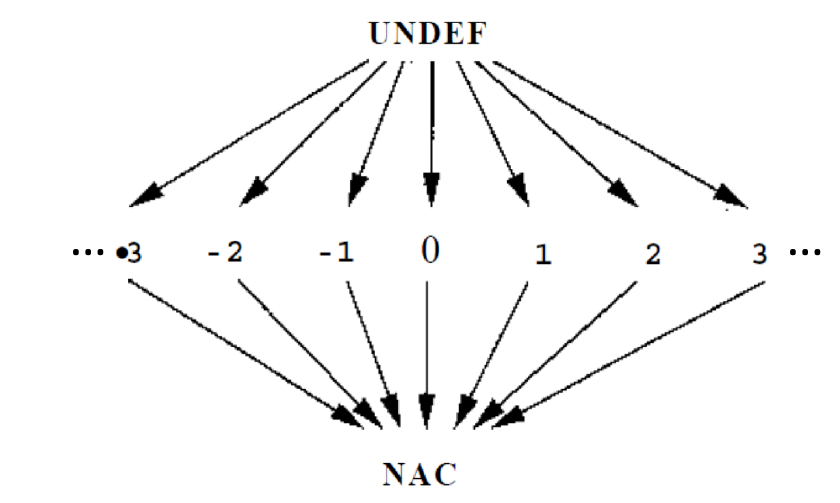
\includegraphics[width=0.3\textwidth]{p19.png}
    \caption{The lattice of constant propogation}
    \label{fig:p19}
\end{figure}


\subsection{Transfer Functions}

Tranfer function dicates how information propagates across a basic block. 
So what we need for our transfer function? \textbf{First}, it must have an identity function which means 
there exists an \(f\) such that \(f(x) = x \) for all \(x\). For example, in Reaching Definitions and Liveness, when 
\(Gen, KILL = \Phi \), this transfer function satisfies \(f(x) = x \). \textbf{Second}, when we compose transfer functions, 
it must be consitent with the transfer function. So if \(f_1,f_2 \in F\), the  \(f_1	\cdot f_2 \in F\).


For example, 
\begin{align*} 
    f_1(x) &= G_1 \cup (x - K_1)\\
    f_2(x) &= G_2 \cup (x - K_2) \\
    f_2(f_1(x)) &= G_2 \cup [(G_1 \cup (x - K_1)) - K_2] \\
    & = [G_2 \cup (G_1 - K_2)] \cup [x-(K_1 \cup K_2)] \\
    G &= G_2 \cup (G_1 - K_2) \\
    K &= K_1 \cup K_2
\end{align*}


\subsection{Monotonicity}


A framework \((F,V,\wedge)\) is monotone if and only if \(x \preceq y \) implies \(f(x) \preceq f(y)\). This means that
a "smaller(more conservative) or equal" input to the same function will always give a "smaller(more conservative)  or equal" output.



Alternatively, \((F,V,\wedge)\) is monotone if and only if \(  f(x \wedge y) \preceq f(x) \wedge f(y)\). So  merge input, then apply \(f\) is small(more conservative)  or equal to apply the transfer
function individually and then merge the result. Values are defined by semi-lattice, the meet operator only ever moves down the lattice from top towards the bottom. 
So we need to constrain the transfer function.

I will show you a unmonotone example.

Let top be 1 and bottom be 0 and the meet operator is \(\cap\). \(f(0) = 1, f(1) = 0\)


Let's check whether reaching definitions is monotone.


Note that monotone framework does not mean \(f(x) \preceq  x\).



\subsection{Distributivity}

Reaching definitions is distributive but constant propogation is not.



\subsection{spped of }

% \[
% f_1(x) = G_1 \cup (x - K_1)   
% f_2(x) = G_2 \cup (x - K_2)
% f_2(f_1(x)) = G_2 \cup [(G_1 \cup (x - K_1)) - K_2] = [G_2 \cup (G_1 - K_2)] \cup [X-(K_1 \cuo K_2)]

% \]




 % The \(\preceq \) not means less or equal to or subset, but it really means lattice inclusion.
% So if \(x \preceq y\), this means x is more conservative or constrained. In another word, x is lattice included in y.





































% Having shown several useful examples of the data-flow abstraction, 
% we now study the family of data-flow schemas as a whole, abstractly. 
% We shall answer several basic questions about data-flow algorithms formally:

% \begin{itemize}

% \item Under what circumstances is the iterative algorithm used in data-flow analysis correct?
% \item How precise is the solution obtained by the iterative algorithm?
% \item Will the iterative algorithm converge?
% \item How fast is the convergence?
% \end{itemize}


% \subsection{Partial Order}\footnote{Based on \url{https://pages.cs.wisc.edu/~horwitz/CS704-NOTES/2.DATAFLOW.html}}

% A binary relation R on a set S is called a partial ordering(poset), or partial order if and only if it is:

% \begin{itemize}
% \item \textbf{Reflexive} \(x \preceq x\)
% \item \textbf{Antisymmetric} if \(x \preceq y\) and \(y \preceq x\) then \(x = y\)
% \item \textbf{Transitive} if \(x \preceq y\) and \(y \preceq z\) then \(x \preceq z\)
% \end{itemize} 



% \subsection{Lattices}

% A lattice is a poset in which every pair of elements has:

% \begin{itemize}
% \item a Least Upper Bound (the join of the two elements), and
% \item a Greatest Lower Bound (the meet of the two elements).
% \end{itemize}    



% \subsection{Complete lattices}


% A complete lattice is a lattice in which all subsets have a greatest lower bound 
% and a least upper bound (the bounds must be in the lattice, but not necessarily 
% in the subsets themselves). Note that Every finite lattice (i.e., S is finite) is complete.


% \subsection{Monotonic and distributive functions}

% A function f: L → L (where L is a lattice) is monotonic iff for all x,y in L: x ⊆ y implies f(x) ⊆ f(y).

% A function f: L → L (where L is a lattice) is distributive iff for all x,y in L: f(x meet y) = f(x) meet f(y).

% Every distributive function is also monotonic (proving that could be good practice!) but not vice versa. For the GEN/KILL dataflow problems, all dataflow functions are distributive. For constant propagation, all functions are monotonic, but not all functions are distributive.


% \subsection{Fixed points}

% x is a fixed point of function f iff f(x) = x.

% \subsection{Meet Operator}


